\documentclass[1p]{elsarticle_modified}
%\bibliographystyle{elsarticle-num}

%\usepackage[colorlinks]{hyperref}
%\usepackage{abbrmath_seonhwa} %\Abb, \Ascr, \Acal ,\Abf, \Afrak
\usepackage{amsfonts}
\usepackage{amssymb}
\usepackage{amsmath}
\usepackage{amsthm}
\usepackage{scalefnt}
\usepackage{amsbsy}
\usepackage{kotex}
\usepackage{caption}
\usepackage{subfig}
\usepackage{color}
\usepackage{graphicx}
\usepackage{xcolor} %% white, black, red, green, blue, cyan, magenta, yellow
\usepackage{float}
\usepackage{setspace}
\usepackage{hyperref}

\usepackage{tikz}
\usetikzlibrary{arrows}

\usepackage{multirow}
\usepackage{array} % fixed length table
\usepackage{hhline}

%%%%%%%%%%%%%%%%%%%%%
\makeatletter
\renewcommand*\env@matrix[1][\arraystretch]{%
	\edef\arraystretch{#1}%
	\hskip -\arraycolsep
	\let\@ifnextchar\new@ifnextchar
	\array{*\c@MaxMatrixCols c}}
\makeatother %https://tex.stackexchange.com/questions/14071/how-can-i-increase-the-line-spacing-in-a-matrix
%%%%%%%%%%%%%%%

\usepackage[normalem]{ulem}

\newcommand{\msout}[1]{\ifmmode\text{\sout{\ensuremath{#1}}}\else\sout{#1}\fi}
%SOURCE: \msout is \stkout macro in https://tex.stackexchange.com/questions/20609/strikeout-in-math-mode

\newcommand{\cancel}[1]{
	\ifmmode
	{\color{red}\msout{#1}}
	\else
	{\color{red}\sout{#1}}
	\fi
}

\newcommand{\add}[1]{
	{\color{blue}\uwave{#1}}
}

\newcommand{\replace}[2]{
	\ifmmode
	{\color{red}\msout{#1}}{\color{blue}\uwave{#2}}
	\else
	{\color{red}\sout{#1}}{\color{blue}\uwave{#2}}
	\fi
}

\newcommand{\Sol}{\mathcal{S}} %segment
\newcommand{\D}{D} %diagram
\newcommand{\A}{\mathcal{A}} %arc


%%%%%%%%%%%%%%%%%%%%%%%%%%%%%5 test

\def\sl{\operatorname{\textup{SL}}(2,\Cbb)}
\def\psl{\operatorname{\textup{PSL}}(2,\Cbb)}
\def\quan{\mkern 1mu \triangleright \mkern 1mu}

\theoremstyle{definition}
\newtheorem{thm}{Theorem}[section]
\newtheorem{prop}[thm]{Proposition}
\newtheorem{lem}[thm]{Lemma}
\newtheorem{ques}[thm]{Question}
\newtheorem{cor}[thm]{Corollary}
\newtheorem{defn}[thm]{Definition}
\newtheorem{exam}[thm]{Example}
\newtheorem{rmk}[thm]{Remark}
\newtheorem{alg}[thm]{Algorithm}

\newcommand{\I}{\sqrt{-1}}
\begin{document}

%\begin{frontmatter}
%
%\title{Boundary parabolic representations of knots up to 8 crossings}
%
%%% Group authors per affiliation:
%\author{Yunhi Cho} 
%\address{Department of Mathematics, University of Seoul, Seoul, Korea}
%\ead{yhcho@uos.ac.kr}
%
%
%\author{Seonhwa Kim} %\fnref{s_kim}}
%\address{Center for Geometry and Physics, Institute for Basic Science, Pohang, 37673, Korea}
%\ead{ryeona17@ibs.re.kr}
%
%\author{Hyuk Kim}
%\address{Department of Mathematical Sciences, Seoul National University, Seoul 08826, Korea}
%\ead{hyukkim@snu.ac.kr}
%
%\author{Seokbeom Yoon}
%\address{Department of Mathematical Sciences, Seoul National University, Seoul, 08826,  Korea}
%\ead{sbyoon15@snu.ac.kr}
%
%\begin{abstract}
%We find all boundary parabolic representation of knots up to 8 crossings.
%
%\end{abstract}
%\begin{keyword}
%    \MSC[2010] 57M25 
%\end{keyword}
%
%\end{frontmatter}

%\linenumbers
%\tableofcontents
%
\newcommand\colored[1]{\textcolor{white}{\rule[-0.35ex]{0.8em}{1.4ex}}\kern-0.8em\color{red} #1}%
%\newcommand\colored[1]{\textcolor{white}{ #1}\kern-2.17ex	\textcolor{white}{ #1}\kern-1.81ex	\textcolor{white}{ #1}\kern-2.15ex\color{red}#1	}

{\Large $\underline{11n_{31}~(K11n_{31})}$}

\setlength{\tabcolsep}{10pt}
\renewcommand{\arraystretch}{1.6}
\vspace{1cm}\begin{tabular}{m{100pt}>{\centering\arraybackslash}m{274pt}}
\multirow{5}{120pt}{
	\centering
	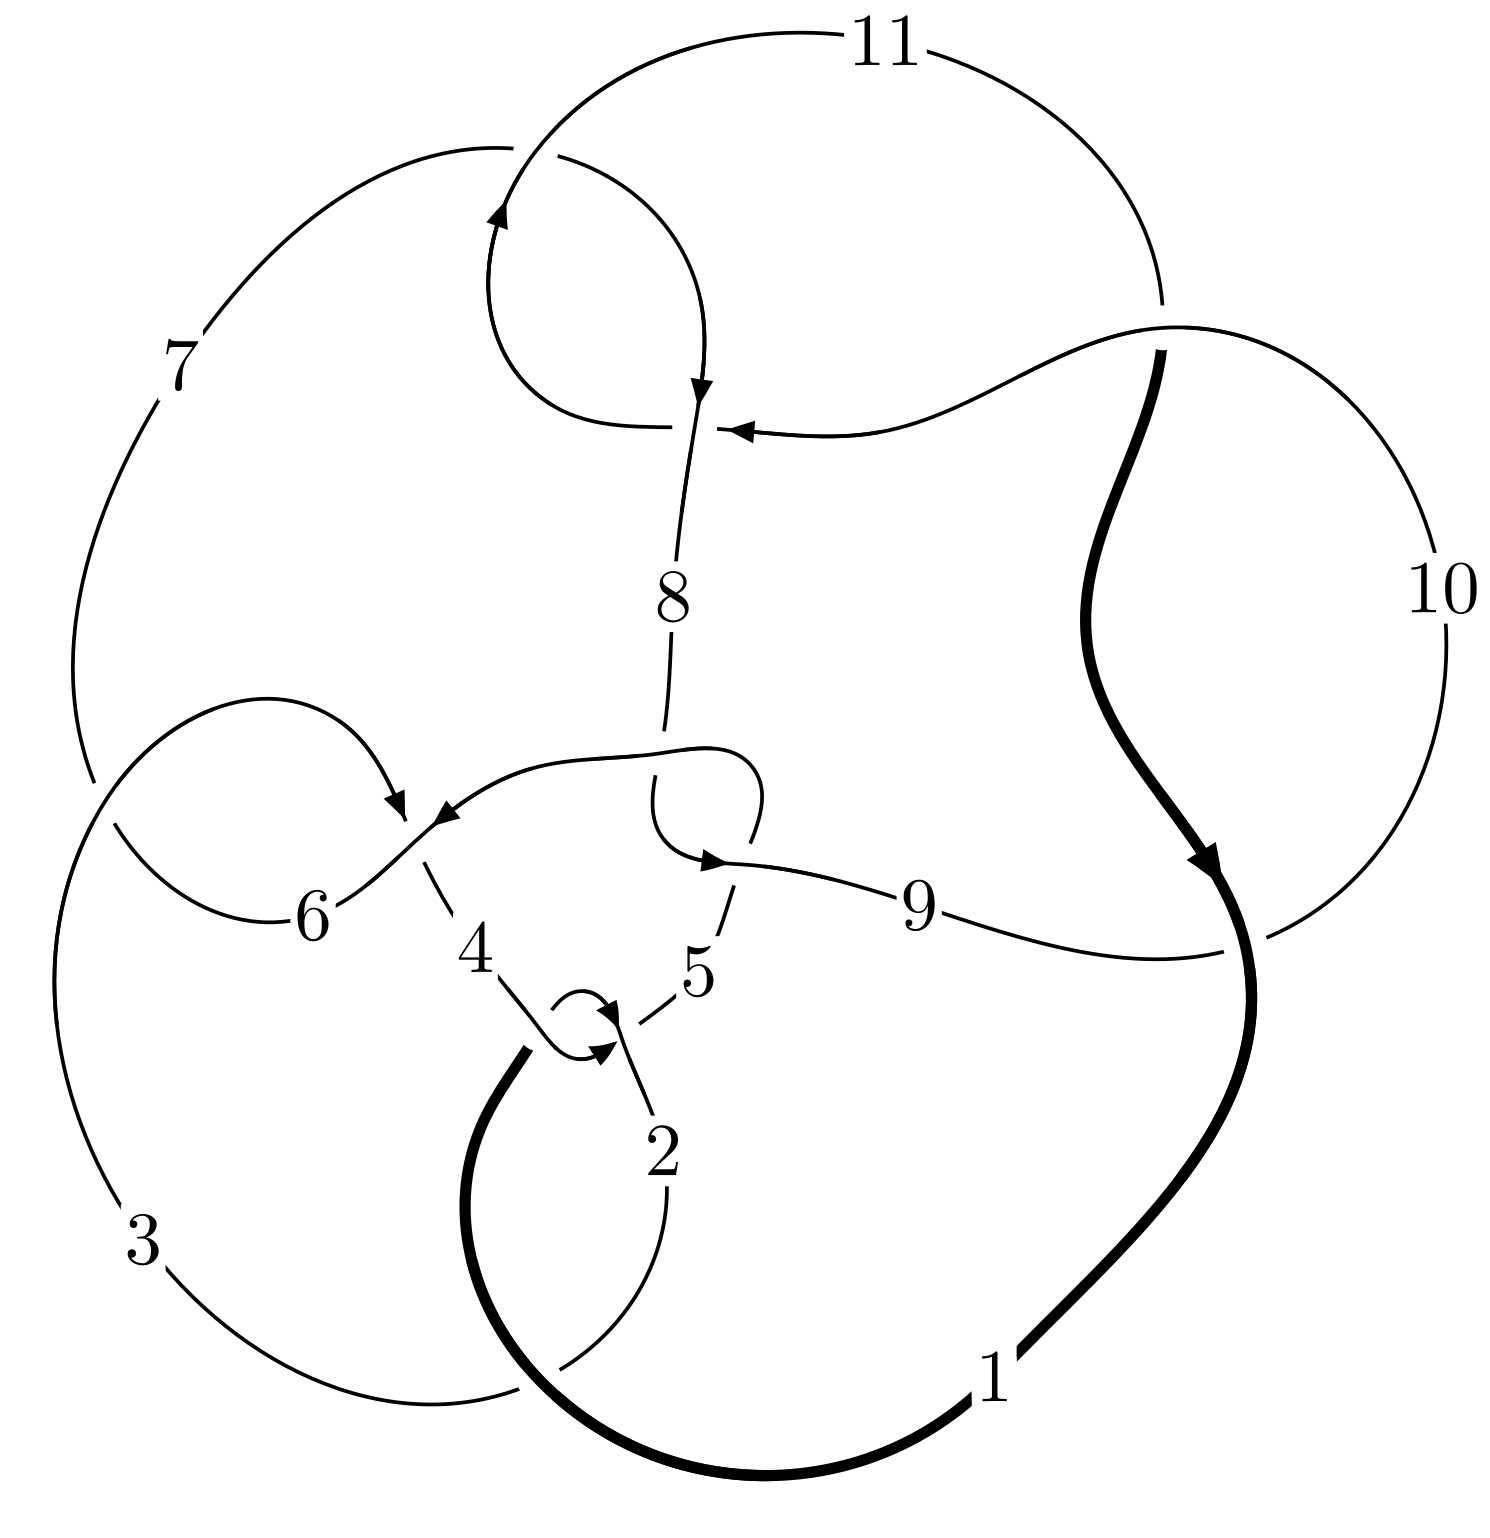
\includegraphics[width=112pt]{../../../GIT/diagram.site/Diagrams/png/647_11n_31.png}\\
\ \ \ A knot diagram\footnotemark}&
\allowdisplaybreaks
\textbf{Linearized knot diagam} \\
\cline{2-2}
 &
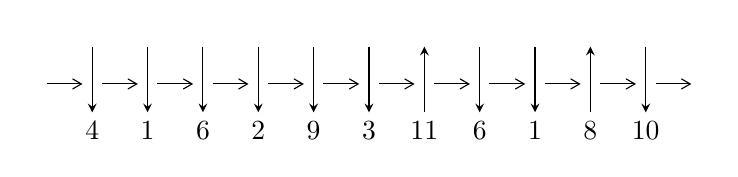
\begin{tikzpicture}[x=20pt, y=17pt]
	% nodes
	\node (C0) at (0, 0) {};
	\node (C1) at (1, 0) {};
	\node (C1U) at (1, +1) {};
	\node (C1D) at (1, -1) {4};

	\node (C2) at (2, 0) {};
	\node (C2U) at (2, +1) {};
	\node (C2D) at (2, -1) {1};

	\node (C3) at (3, 0) {};
	\node (C3U) at (3, +1) {};
	\node (C3D) at (3, -1) {6};

	\node (C4) at (4, 0) {};
	\node (C4U) at (4, +1) {};
	\node (C4D) at (4, -1) {2};

	\node (C5) at (5, 0) {};
	\node (C5U) at (5, +1) {};
	\node (C5D) at (5, -1) {9};

	\node (C6) at (6, 0) {};
	\node (C6U) at (6, +1) {};
	\node (C6D) at (6, -1) {3};

	\node (C7) at (7, 0) {};
	\node (C7U) at (7, +1) {};
	\node (C7D) at (7, -1) {11};

	\node (C8) at (8, 0) {};
	\node (C8U) at (8, +1) {};
	\node (C8D) at (8, -1) {6};

	\node (C9) at (9, 0) {};
	\node (C9U) at (9, +1) {};
	\node (C9D) at (9, -1) {1};

	\node (C10) at (10, 0) {};
	\node (C10U) at (10, +1) {};
	\node (C10D) at (10, -1) {8};

	\node (C11) at (11, 0) {};
	\node (C11U) at (11, +1) {};
	\node (C11D) at (11, -1) {10};
	\node (C12) at (12, 0) {};

	% arrows
	\draw[->,>={angle 60}]
	(C0) edge (C1) (C1) edge (C2) (C2) edge (C3) (C3) edge (C4) (C4) edge (C5) (C5) edge (C6) (C6) edge (C7) (C7) edge (C8) (C8) edge (C9) (C9) edge (C10) (C10) edge (C11) (C11) edge (C12) ;	\draw[->,>=stealth]
	(C1U) edge (C1D) (C2U) edge (C2D) (C3U) edge (C3D) (C4U) edge (C4D) (C5U) edge (C5D) (C6U) edge (C6D) (C7D) edge (C7U) (C8U) edge (C8D) (C9U) edge (C9D) (C10D) edge (C10U) (C11U) edge (C11D) ;
	\end{tikzpicture} \\
\hhline{~~} \\& 
\textbf{Solving Sequence} \\ \cline{2-2} 
 &
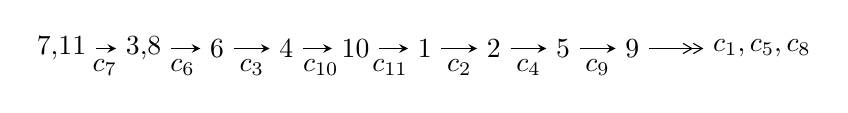
\begin{tikzpicture}[x=25pt, y=7pt]
	% node
	\node (A0) at (-1/8, 0) {7,11};
	\node (A1) at (17/16, 0) {3,8};
	\node (A2) at (17/8, 0) {6};
	\node (A3) at (25/8, 0) {4};
	\node (A4) at (33/8, 0) {10};
	\node (A5) at (41/8, 0) {1};
	\node (A6) at (49/8, 0) {2};
	\node (A7) at (57/8, 0) {5};
	\node (A8) at (65/8, 0) {9};
	\node (C1) at (1/2, -1) {$c_{7}$};
	\node (C2) at (13/8, -1) {$c_{6}$};
	\node (C3) at (21/8, -1) {$c_{3}$};
	\node (C4) at (29/8, -1) {$c_{10}$};
	\node (C5) at (37/8, -1) {$c_{11}$};
	\node (C6) at (45/8, -1) {$c_{2}$};
	\node (C7) at (53/8, -1) {$c_{4}$};
	\node (C8) at (61/8, -1) {$c_{9}$};
	\node (A9) at (10, 0) {$c_{1},c_{5},c_{8}$};

	% edge
	\draw[->,>=stealth]	
	(A0) edge (A1) (A1) edge (A2) (A2) edge (A3) (A3) edge (A4) (A4) edge (A5) (A5) edge (A6) (A6) edge (A7) (A7) edge (A8) ;
	\draw[->>,>={angle 60}]	
	(A8) edge (A9);
\end{tikzpicture} \\ 

\end{tabular} \\

\footnotetext{
The image of knot diagram is generated by the software ``\textbf{Draw programme}" developed by Andrew Bartholomew(\url{http://www.layer8.co.uk/maths/draw/index.htm\#Running-draw}), where we modified some parts for our purpose(\url{https://github.com/CATsTAILs/LinksPainter}).
}\phantom \\ \newline 
\centering \textbf{Ideals for irreducible components\footnotemark of $X_{\text{par}}$} 
 
\begin{align*}
I^u_{1}&=\langle 
7 u^{10}-8 u^9-23 u^8+57 u^7-2 u^6+8 u^5-87 u^4+232 u^3+3 u^2+164 b+47 u-106,\\
\phantom{I^u_{1}}&\phantom{= \langle  }38 u^{10}-184 u^9+414 u^8-493 u^7+446 u^6-513 u^5+828 u^4-650 u^3+397 u^2+82 a-395 u+350,\\
\phantom{I^u_{1}}&\phantom{= \langle  }u^{11}-5 u^{10}+12 u^9-16 u^8+16 u^7-17 u^6+25 u^5-21 u^4+14 u^3-10 u^2+10 u-1\rangle \\
I^u_{2}&=\langle 
- a^2 u-2 a u+b- a+u,\;a^3- a^2 u+2 a^2- a u- a+u-2,\;u^2+u+1\rangle \\
I^u_{3}&=\langle 
b,\;- u^3+2 u^2+a-2 u,\;u^4- u^3+u^2+1\rangle \\
\\
\end{align*}
\raggedright * 3 irreducible components of $\dim_{\mathbb{C}}=0$, with total 21 representations.\\
\footnotetext{All coefficients of polynomials are rational numbers. But the coefficients are sometimes approximated in decimal forms when there is not enough margin.}
\newpage
\renewcommand{\arraystretch}{1}
\centering \section*{I. $I^u_{1}= \langle 7 u^{10}-8 u^9+\cdots+164 b-106,\;38 u^{10}-184 u^9+\cdots+82 a+350,\;u^{11}-5 u^{10}+\cdots+10 u-1 \rangle$}
\flushleft \textbf{(i) Arc colorings}\\
\begin{tabular}{m{7pt} m{180pt} m{7pt} m{180pt} }
\flushright $a_{7}=$&$\begin{pmatrix}1\\0\end{pmatrix}$ \\
\flushright $a_{11}=$&$\begin{pmatrix}0\\u\end{pmatrix}$ \\
\flushright $a_{3}=$&$\begin{pmatrix}-0.463415 u^{10}+2.24390 u^{9}+\cdots+4.81707 u-4.26829\\-0.0426829 u^{10}+0.0487805 u^{9}+\cdots-0.286585 u+0.646341\end{pmatrix}$ \\
\flushright $a_{8}=$&$\begin{pmatrix}1\\- u^2\end{pmatrix}$ \\
\flushright $a_{6}=$&$\begin{pmatrix}0.359756 u^{10}-1.76829 u^{9}+\cdots-3.79878 u+3.69512\\0.0121951 u^{10}+0.164634 u^{9}+\cdots+1.18902 u-0.506098\end{pmatrix}$ \\
\flushright $a_{4}=$&$\begin{pmatrix}-0.871951 u^{10}+3.85366 u^{9}+\cdots+6.35976 u-6.43902\\0.884146 u^{10}-3.68902 u^{9}+\cdots-5.67073 u+1.43293\end{pmatrix}$ \\
\flushright $a_{10}=$&$\begin{pmatrix}- u\\u^3+u\end{pmatrix}$ \\
\flushright $a_{1}=$&$\begin{pmatrix}- u^3\\u^5+u^3+u\end{pmatrix}$ \\
\flushright $a_{2}=$&$\begin{pmatrix}-0.152439 u^{10}+1.31707 u^{9}+\cdots+2.76220 u-4.04878\\-1.23780 u^{10}+5.41463 u^{9}+\cdots+8.68902 u-0.256098\end{pmatrix}$ \\
\flushright $a_{5}=$&$\begin{pmatrix}-0.201220 u^{10}+1.15854 u^{9}+\cdots+2.00610 u-3.52439\\-0.195122 u^{10}+3.11585 u^{9}+\cdots+5.22561 u-0.152439\end{pmatrix}$ \\
\flushright $a_{9}=$&$\begin{pmatrix}- u^5- u\\u^7+u^5+2 u^3+u\end{pmatrix}$\\ \flushright $a_{9}=$&$\begin{pmatrix}- u^5- u\\u^7+u^5+2 u^3+u\end{pmatrix}$\\&\end{tabular}
\flushleft \textbf{(ii) Obstruction class $= -1$}\\~\\
\flushleft \textbf{(iii) Cusp Shapes $= -\frac{69}{82} u^{10}+\frac{319}{82} u^9-\frac{364}{41} u^8+\frac{460}{41} u^7-\frac{935}{82} u^6+\frac{476}{41} u^5-\frac{687}{41} u^4+\frac{520}{41} u^3-\frac{539}{41} u^2+\frac{673}{82} u-\frac{444}{41}$}\\~\\
\newpage\renewcommand{\arraystretch}{1}
\flushleft \textbf{(iv) u-Polynomials at the component}\newline \\
\begin{tabular}{m{50pt}|m{274pt}}
Crossings & \hspace{64pt}u-Polynomials at each crossing \\
\hline $$\begin{aligned}c_{1},c_{4}\end{aligned}$$&$\begin{aligned}
&u^{11}-7 u^{10}+\cdots-9 u+1
\end{aligned}$\\
\hline $$\begin{aligned}c_{2}\end{aligned}$$&$\begin{aligned}
&u^{11}+11 u^{10}+\cdots+5 u+1
\end{aligned}$\\
\hline $$\begin{aligned}c_{3},c_{6}\end{aligned}$$&$\begin{aligned}
&u^{11}-6 u^{10}+\cdots-24 u+16
\end{aligned}$\\
\hline $$\begin{aligned}c_{5},c_{8}\end{aligned}$$&$\begin{aligned}
&u^{11}-2 u^{10}+\cdots+96 u+64
\end{aligned}$\\
\hline $$\begin{aligned}c_{7},c_{10}\end{aligned}$$&$\begin{aligned}
&u^{11}+5 u^{10}+\cdots+10 u+1
\end{aligned}$\\
\hline $$\begin{aligned}c_{9},c_{11}\end{aligned}$$&$\begin{aligned}
&u^{11}- u^{10}+\cdots+80 u-1
\end{aligned}$\\
\hline
\end{tabular}\\~\\
\newpage\renewcommand{\arraystretch}{1}
\flushleft \textbf{(v) Riley Polynomials at the component}\newline \\
\begin{tabular}{m{50pt}|m{274pt}}
Crossings & \hspace{64pt}Riley Polynomials at each crossing \\
\hline $$\begin{aligned}c_{1},c_{4}\end{aligned}$$&$\begin{aligned}
&y^{11}-11 y^{10}+\cdots+5 y-1
\end{aligned}$\\
\hline $$\begin{aligned}c_{2}\end{aligned}$$&$\begin{aligned}
&y^{11}+113 y^{10}+\cdots-3895 y-1
\end{aligned}$\\
\hline $$\begin{aligned}c_{3},c_{6}\end{aligned}$$&$\begin{aligned}
&y^{11}+30 y^{10}+\cdots-2240 y-256
\end{aligned}$\\
\hline $$\begin{aligned}c_{5},c_{8}\end{aligned}$$&$\begin{aligned}
&y^{11}+52 y^{10}+\cdots+33792 y-4096
\end{aligned}$\\
\hline $$\begin{aligned}c_{7},c_{10}\end{aligned}$$&$\begin{aligned}
&y^{11}- y^{10}+\cdots+80 y-1
\end{aligned}$\\
\hline $$\begin{aligned}c_{9},c_{11}\end{aligned}$$&$\begin{aligned}
&y^{11}+31 y^{10}+\cdots+6676 y-1
\end{aligned}$\\
\hline
\end{tabular}\\~\\
\newpage\flushleft \textbf{(vi) Complex Volumes and Cusp Shapes}
$$\begin{array}{c|c|c}  
\text{Solutions to }I^u_{1}& \I (\text{vol} + \sqrt{-1}CS) & \text{Cusp shape}\\
 \hline 
\begin{aligned}
u &= -0.685415 + 0.773477 I \\
a &= -0.73400 + 2.17133 I \\
b &= -0.460151 - 0.697009 I\end{aligned}
 & -1.32886 - 1.52951 I & -7.26885 + 4.94950 I \\ \hline\begin{aligned}
u &= -0.685415 - 0.773477 I \\
a &= -0.73400 - 2.17133 I \\
b &= -0.460151 + 0.697009 I\end{aligned}
 & -1.32886 + 1.52951 I & -7.26885 - 4.94950 I \\ \hline\begin{aligned}
u &= \phantom{-}0.855917 + 0.653801 I \\
a &= \phantom{-}0.594255 + 0.858681 I \\
b &= \phantom{-}0.710923 - 1.191110 I\end{aligned}
 & \phantom{-}4.33457 + 4.30583 I & -3.61862 - 3.76799 I \\ \hline\begin{aligned}
u &= \phantom{-}0.855917 - 0.653801 I \\
a &= \phantom{-}0.594255 - 0.858681 I \\
b &= \phantom{-}0.710923 + 1.191110 I\end{aligned}
 & \phantom{-}4.33457 - 4.30583 I & -3.61862 + 3.76799 I \\ \hline\begin{aligned}
u &= -0.315247 + 0.806810 I \\
a &= -0.545836 + 0.331424 I \\
b &= -0.143998 + 0.360224 I\end{aligned}
 & -0.33628 - 1.50726 I & -2.98443 + 4.38710 I \\ \hline\begin{aligned}
u &= -0.315247 - 0.806810 I \\
a &= -0.545836 - 0.331424 I \\
b &= -0.143998 - 0.360224 I\end{aligned}
 & -0.33628 + 1.50726 I & -2.98443 - 4.38710 I \\ \hline\begin{aligned}
u &= \phantom{-}0.94424 + 1.31822 I \\
a &= -1.30445 - 1.00484 I \\
b &= -1.48748 + 2.15268 I\end{aligned}
 & -18.0782 + 10.5314 I & -5.95863 - 4.05407 I \\ \hline\begin{aligned}
u &= \phantom{-}0.94424 - 1.31822 I \\
a &= -1.30445 + 1.00484 I \\
b &= -1.48748 - 2.15268 I\end{aligned}
 & -18.0782 - 10.5314 I & -5.95863 + 4.05407 I \\ \hline\begin{aligned}
u &= \phantom{-}0.110617\phantom{ +0.000000I} \\
a &= -3.78537\phantom{ +0.000000I} \\
b &= \phantom{-}0.612580\phantom{ +0.000000I}\end{aligned}
 & -1.00288\phantom{ +0.000000I} & -10.0670\phantom{ +0.000000I} \\ \hline\begin{aligned}
u &= \phantom{-}1.64519 + 0.99588 I \\
a &= \phantom{-}0.882711 + 0.513382 I \\
b &= -1.92558 - 3.89584 I\end{aligned}
 & -16.1660 - 1.6365 I & -5.13576 + 0.13357 I\\
 \hline 
 \end{array}$$\newpage$$\begin{array}{c|c|c}  
\text{Solutions to }I^u_{1}& \I (\text{vol} + \sqrt{-1}CS) & \text{Cusp shape}\\
 \hline 
\begin{aligned}
u &= \phantom{-}1.64519 - 0.99588 I \\
a &= \phantom{-}0.882711 - 0.513382 I \\
b &= -1.92558 + 3.89584 I\end{aligned}
 & -16.1660 + 1.6365 I & -5.13576 - 0.13357 I\\
 \hline 
 \end{array}$$\newpage\newpage\renewcommand{\arraystretch}{1}
\centering \section*{II. $I^u_{2}= \langle - a^2 u-2 a u+b- a+u,\;a^3- a^2 u+2 a^2- a u- a+u-2,\;u^2+u+1 \rangle$}
\flushleft \textbf{(i) Arc colorings}\\
\begin{tabular}{m{7pt} m{180pt} m{7pt} m{180pt} }
\flushright $a_{7}=$&$\begin{pmatrix}1\\0\end{pmatrix}$ \\
\flushright $a_{11}=$&$\begin{pmatrix}0\\u\end{pmatrix}$ \\
\flushright $a_{3}=$&$\begin{pmatrix}a\\a^2 u+2 a u+a- u\end{pmatrix}$ \\
\flushright $a_{8}=$&$\begin{pmatrix}1\\u+1\end{pmatrix}$ \\
\flushright $a_{6}=$&$\begin{pmatrix}a^2 u+a u+a-3 u\\- a^2+a u+3\end{pmatrix}$ \\
\flushright $a_{4}=$&$\begin{pmatrix}- a^2 u-2 a^2- a u-2 a+2\\- a^2 u- a^2- a u- a+u+2\end{pmatrix}$ \\
\flushright $a_{10}=$&$\begin{pmatrix}- u\\u+1\end{pmatrix}$ \\
\flushright $a_{1}=$&$\begin{pmatrix}-1\\0\end{pmatrix}$ \\
\flushright $a_{2}=$&$\begin{pmatrix}a^2 u+2 a u+2 a- u\\a^2 u+2 a u+a- u\end{pmatrix}$ \\
\flushright $a_{5}=$&$\begin{pmatrix}a^2 u+a u+a-3 u\\- a^2+a u+3\end{pmatrix}$ \\
\flushright $a_{9}=$&$\begin{pmatrix}1\\u+1\end{pmatrix}$\\ \flushright $a_{9}=$&$\begin{pmatrix}1\\u+1\end{pmatrix}$\\&\end{tabular}
\flushleft \textbf{(ii) Obstruction class $= 1$}\\~\\
\flushleft \textbf{(iii) Cusp Shapes $= -4 a^2-2 a u- a-1$}\\~\\
\newpage\renewcommand{\arraystretch}{1}
\flushleft \textbf{(iv) u-Polynomials at the component}\newline \\
\begin{tabular}{m{50pt}|m{274pt}}
Crossings & \hspace{64pt}u-Polynomials at each crossing \\
\hline $$\begin{aligned}c_{1}\end{aligned}$$&$\begin{aligned}
&(u^3+u^2-1)^2
\end{aligned}$\\
\hline $$\begin{aligned}c_{2},c_{6}\end{aligned}$$&$\begin{aligned}
&(u^3+u^2+2 u+1)^2
\end{aligned}$\\
\hline $$\begin{aligned}c_{3}\end{aligned}$$&$\begin{aligned}
&(u^3- u^2+2 u-1)^2
\end{aligned}$\\
\hline $$\begin{aligned}c_{4}\end{aligned}$$&$\begin{aligned}
&(u^3- u^2+1)^2
\end{aligned}$\\
\hline $$\begin{aligned}c_{5},c_{8}\end{aligned}$$&$\begin{aligned}
&u^6
\end{aligned}$\\
\hline $$\begin{aligned}c_{7},c_{11}\end{aligned}$$&$\begin{aligned}
&(u^2+u+1)^3
\end{aligned}$\\
\hline $$\begin{aligned}c_{9},c_{10}\end{aligned}$$&$\begin{aligned}
&(u^2- u+1)^3
\end{aligned}$\\
\hline
\end{tabular}\\~\\
\newpage\renewcommand{\arraystretch}{1}
\flushleft \textbf{(v) Riley Polynomials at the component}\newline \\
\begin{tabular}{m{50pt}|m{274pt}}
Crossings & \hspace{64pt}Riley Polynomials at each crossing \\
\hline $$\begin{aligned}c_{1},c_{4}\end{aligned}$$&$\begin{aligned}
&(y^3- y^2+2 y-1)^2
\end{aligned}$\\
\hline $$\begin{aligned}c_{2},c_{3},c_{6}\end{aligned}$$&$\begin{aligned}
&(y^3+3 y^2+2 y-1)^2
\end{aligned}$\\
\hline $$\begin{aligned}c_{5},c_{8}\end{aligned}$$&$\begin{aligned}
&y^6
\end{aligned}$\\
\hline $$\begin{aligned}c_{7},c_{9},c_{10}\\c_{11}\end{aligned}$$&$\begin{aligned}
&(y^2+y+1)^3
\end{aligned}$\\
\hline
\end{tabular}\\~\\
\newpage\flushleft \textbf{(vi) Complex Volumes and Cusp Shapes}
$$\begin{array}{c|c|c}  
\text{Solutions to }I^u_{2}& \I (\text{vol} + \sqrt{-1}CS) & \text{Cusp shape}\\
 \hline 
\begin{aligned}
u &= -0.500000 + 0.866025 I \\
a &= \phantom{-}0.901916 + 0.094973 I \\
b &= -0.215080 + 1.307140 I\end{aligned}
 & \phantom{-}3.02413 + 0.79824 I & -4.05323 - 2.24743 I \\ \hline\begin{aligned}
u &= -0.500000 + 0.866025 I \\
a &= -1.362120 + 0.277556 I \\
b &= -0.215080 - 1.307140 I\end{aligned}
 & \phantom{-}3.02413 - 4.85801 I & -7.63258 + 5.38377 I \\ \hline\begin{aligned}
u &= -0.500000 + 0.866025 I \\
a &= -2.03980 + 0.49350 I \\
b &= -0.569840\phantom{ +0.000000I}\end{aligned}
 & -1.11345 - 2.02988 I & -15.8142 + 11.5861 I \\ \hline\begin{aligned}
u &= -0.500000 - 0.866025 I \\
a &= \phantom{-}0.901916 - 0.094973 I \\
b &= -0.215080 - 1.307140 I\end{aligned}
 & \phantom{-}3.02413 - 0.79824 I & -4.05323 + 2.24743 I \\ \hline\begin{aligned}
u &= -0.500000 - 0.866025 I \\
a &= -1.362120 - 0.277556 I \\
b &= -0.215080 + 1.307140 I\end{aligned}
 & \phantom{-}3.02413 + 4.85801 I & -7.63258 - 5.38377 I \\ \hline\begin{aligned}
u &= -0.500000 - 0.866025 I \\
a &= -2.03980 - 0.49350 I \\
b &= -0.569840\phantom{ +0.000000I}\end{aligned}
 & -1.11345 + 2.02988 I & -15.8142 - 11.5861 I\\
 \hline 
 \end{array}$$\newpage\newpage\renewcommand{\arraystretch}{1}
\centering \section*{III. $I^u_{3}= \langle b,\;- u^3+2 u^2+a-2 u,\;u^4- u^3+u^2+1 \rangle$}
\flushleft \textbf{(i) Arc colorings}\\
\begin{tabular}{m{7pt} m{180pt} m{7pt} m{180pt} }
\flushright $a_{7}=$&$\begin{pmatrix}1\\0\end{pmatrix}$ \\
\flushright $a_{11}=$&$\begin{pmatrix}0\\u\end{pmatrix}$ \\
\flushright $a_{3}=$&$\begin{pmatrix}u^3-2 u^2+2 u\\0\end{pmatrix}$ \\
\flushright $a_{8}=$&$\begin{pmatrix}1\\- u^2\end{pmatrix}$ \\
\flushright $a_{6}=$&$\begin{pmatrix}1\\0\end{pmatrix}$ \\
\flushright $a_{4}=$&$\begin{pmatrix}u^3-2 u^2+2 u\\0\end{pmatrix}$ \\
\flushright $a_{10}=$&$\begin{pmatrix}- u\\u^3+u\end{pmatrix}$ \\
\flushright $a_{1}=$&$\begin{pmatrix}- u^3\\u^3- u^2-1\end{pmatrix}$ \\
\flushright $a_{2}=$&$\begin{pmatrix}-2 u^2+2 u\\u^3- u^2-1\end{pmatrix}$ \\
\flushright $a_{5}=$&$\begin{pmatrix}u^3\\- u^3+u^2+1\end{pmatrix}$ \\
\flushright $a_{9}=$&$\begin{pmatrix}u^2+1\\- u^2\end{pmatrix}$\\ \flushright $a_{9}=$&$\begin{pmatrix}u^2+1\\- u^2\end{pmatrix}$\\&\end{tabular}
\flushleft \textbf{(ii) Obstruction class $= 1$}\\~\\
\flushleft \textbf{(iii) Cusp Shapes $= -3 u^3-3 u^2+8 u-12$}\\~\\
\newpage\renewcommand{\arraystretch}{1}
\flushleft \textbf{(iv) u-Polynomials at the component}\newline \\
\begin{tabular}{m{50pt}|m{274pt}}
Crossings & \hspace{64pt}u-Polynomials at each crossing \\
\hline $$\begin{aligned}c_{1}\end{aligned}$$&$\begin{aligned}
&(u-1)^4
\end{aligned}$\\
\hline $$\begin{aligned}c_{2},c_{4}\end{aligned}$$&$\begin{aligned}
&(u+1)^4
\end{aligned}$\\
\hline $$\begin{aligned}c_{3},c_{6}\end{aligned}$$&$\begin{aligned}
&u^4
\end{aligned}$\\
\hline $$\begin{aligned}c_{5},c_{9}\end{aligned}$$&$\begin{aligned}
&u^4- u^3+3 u^2-2 u+1
\end{aligned}$\\
\hline $$\begin{aligned}c_{7}\end{aligned}$$&$\begin{aligned}
&u^4- u^3+u^2+1
\end{aligned}$\\
\hline $$\begin{aligned}c_{8},c_{11}\end{aligned}$$&$\begin{aligned}
&u^4+u^3+3 u^2+2 u+1
\end{aligned}$\\
\hline $$\begin{aligned}c_{10}\end{aligned}$$&$\begin{aligned}
&u^4+u^3+u^2+1
\end{aligned}$\\
\hline
\end{tabular}\\~\\
\newpage\renewcommand{\arraystretch}{1}
\flushleft \textbf{(v) Riley Polynomials at the component}\newline \\
\begin{tabular}{m{50pt}|m{274pt}}
Crossings & \hspace{64pt}Riley Polynomials at each crossing \\
\hline $$\begin{aligned}c_{1},c_{2},c_{4}\end{aligned}$$&$\begin{aligned}
&(y-1)^4
\end{aligned}$\\
\hline $$\begin{aligned}c_{3},c_{6}\end{aligned}$$&$\begin{aligned}
&y^4
\end{aligned}$\\
\hline $$\begin{aligned}c_{5},c_{8},c_{9}\\c_{11}\end{aligned}$$&$\begin{aligned}
&y^4+5 y^3+7 y^2+2 y+1
\end{aligned}$\\
\hline $$\begin{aligned}c_{7},c_{10}\end{aligned}$$&$\begin{aligned}
&y^4+y^3+3 y^2+2 y+1
\end{aligned}$\\
\hline
\end{tabular}\\~\\
\newpage\flushleft \textbf{(vi) Complex Volumes and Cusp Shapes}
$$\begin{array}{c|c|c}  
\text{Solutions to }I^u_{3}& \I (\text{vol} + \sqrt{-1}CS) & \text{Cusp shape}\\
 \hline 
\begin{aligned}
u &= -0.351808 + 0.720342 I \\
a &= \phantom{-}0.59074 + 2.34806 I \\
b &= \phantom{-0.000000 } 0\end{aligned}
 & -1.85594 - 1.41510 I & -15.1414 + 7.6022 I \\ \hline\begin{aligned}
u &= -0.351808 - 0.720342 I \\
a &= \phantom{-}0.59074 - 2.34806 I \\
b &= \phantom{-0.000000 } 0\end{aligned}
 & -1.85594 + 1.41510 I & -15.1414 - 7.6022 I \\ \hline\begin{aligned}
u &= \phantom{-}0.851808 + 0.911292 I \\
a &= \phantom{-}0.409261 - 0.055548 I \\
b &= \phantom{-0.000000 } 0\end{aligned}
 & \phantom{-}5.14581 + 3.16396 I & -0.358581 - 1.047693 I \\ \hline\begin{aligned}
u &= \phantom{-}0.851808 - 0.911292 I \\
a &= \phantom{-}0.409261 + 0.055548 I \\
b &= \phantom{-0.000000 } 0\end{aligned}
 & \phantom{-}5.14581 - 3.16396 I & -0.358581 + 1.047693 I\\
 \hline 
 \end{array}$$\newpage
\newpage\renewcommand{\arraystretch}{1}
\centering \section*{ IV. u-Polynomials}
\begin{tabular}{m{50pt}|m{274pt}}
Crossings & \hspace{64pt}u-Polynomials at each crossing \\
\hline $$\begin{aligned}c_{1}\end{aligned}$$&$\begin{aligned}
&((u-1)^4)(u^3+u^2-1)^2(u^{11}-7 u^{10}+\cdots-9 u+1)
\end{aligned}$\\
\hline $$\begin{aligned}c_{2}\end{aligned}$$&$\begin{aligned}
&((u+1)^4)(u^3+u^2+2 u+1)^2(u^{11}+11 u^{10}+\cdots+5 u+1)
\end{aligned}$\\
\hline $$\begin{aligned}c_{3}\end{aligned}$$&$\begin{aligned}
&u^4(u^3- u^2+2 u-1)^2(u^{11}-6 u^{10}+\cdots-24 u+16)
\end{aligned}$\\
\hline $$\begin{aligned}c_{4}\end{aligned}$$&$\begin{aligned}
&((u+1)^4)(u^3- u^2+1)^2(u^{11}-7 u^{10}+\cdots-9 u+1)
\end{aligned}$\\
\hline $$\begin{aligned}c_{5}\end{aligned}$$&$\begin{aligned}
&u^6(u^4- u^3+3 u^2-2 u+1)(u^{11}-2 u^{10}+\cdots+96 u+64)
\end{aligned}$\\
\hline $$\begin{aligned}c_{6}\end{aligned}$$&$\begin{aligned}
&u^4(u^3+u^2+2 u+1)^2(u^{11}-6 u^{10}+\cdots-24 u+16)
\end{aligned}$\\
\hline $$\begin{aligned}c_{7}\end{aligned}$$&$\begin{aligned}
&((u^2+u+1)^3)(u^4- u^3+u^2+1)(u^{11}+5 u^{10}+\cdots+10 u+1)
\end{aligned}$\\
\hline $$\begin{aligned}c_{8}\end{aligned}$$&$\begin{aligned}
&u^6(u^4+u^3+3 u^2+2 u+1)(u^{11}-2 u^{10}+\cdots+96 u+64)
\end{aligned}$\\
\hline $$\begin{aligned}c_{9}\end{aligned}$$&$\begin{aligned}
&((u^2- u+1)^3)(u^4- u^3+3 u^2-2 u+1)(u^{11}- u^{10}+\cdots+80 u-1)
\end{aligned}$\\
\hline $$\begin{aligned}c_{10}\end{aligned}$$&$\begin{aligned}
&((u^2- u+1)^3)(u^4+u^3+u^2+1)(u^{11}+5 u^{10}+\cdots+10 u+1)
\end{aligned}$\\
\hline $$\begin{aligned}c_{11}\end{aligned}$$&$\begin{aligned}
&((u^2+u+1)^3)(u^4+u^3+3 u^2+2 u+1)(u^{11}- u^{10}+\cdots+80 u-1)
\end{aligned}$\\
\hline
\end{tabular}\newpage\renewcommand{\arraystretch}{1}
\centering \section*{ V. Riley Polynomials}
\begin{tabular}{m{50pt}|m{274pt}}
Crossings & \hspace{64pt}Riley Polynomials at each crossing \\
\hline $$\begin{aligned}c_{1},c_{4}\end{aligned}$$&$\begin{aligned}
&((y-1)^4)(y^3- y^2+2 y-1)^2(y^{11}-11 y^{10}+\cdots+5 y-1)
\end{aligned}$\\
\hline $$\begin{aligned}c_{2}\end{aligned}$$&$\begin{aligned}
&((y-1)^4)(y^3+3 y^2+2 y-1)^2(y^{11}+113 y^{10}+\cdots-3895 y-1)
\end{aligned}$\\
\hline $$\begin{aligned}c_{3},c_{6}\end{aligned}$$&$\begin{aligned}
&y^4(y^3+3 y^2+2 y-1)^2(y^{11}+30 y^{10}+\cdots-2240 y-256)
\end{aligned}$\\
\hline $$\begin{aligned}c_{5},c_{8}\end{aligned}$$&$\begin{aligned}
&y^6(y^4+5 y^3+\cdots+2 y+1)(y^{11}+52 y^{10}+\cdots+33792 y-4096)
\end{aligned}$\\
\hline $$\begin{aligned}c_{7},c_{10}\end{aligned}$$&$\begin{aligned}
&((y^2+y+1)^3)(y^4+y^3+3 y^2+2 y+1)(y^{11}- y^{10}+\cdots+80 y-1)
\end{aligned}$\\
\hline $$\begin{aligned}c_{9},c_{11}\end{aligned}$$&$\begin{aligned}
&((y^2+y+1)^3)(y^4+5 y^3+\cdots+2 y+1)(y^{11}+31 y^{10}+\cdots+6676 y-1)
\end{aligned}$\\
\hline
\end{tabular}
\vskip 2pc
\end{document}